% Part: history
% Chapter: set-theory
% Section: limits

\documentclass[../../../include/open-logic-section]{subfiles}

\begin{document}

\olfileid{his}{set}{limits}

\olsection{সীমার কঠোর সংজ্ঞা}

আজকাল আগের সমস্যাটির প্রমিত সমাধান হলো
অতিক্ষুদ্র রাশির ব্যবহার বাদ দেওয়া। পদ্ধতিটি
এমন।

$\beta$ যত ছোট হতে থাকে, আমরা ঢালের
তত ভালো কাছাকাছি মান পাই—এটি দেখেছি।
% BN-SRC-487: the varying difference quotient, not the fixed f'(c), tends to the gradient.
বস্তুত, $\beta$ যত ইচ্ছা $0$-এর কাছে
এলে ভাগফল
$\frac{f(c+\beta)-f(c)}{\beta}$-এর মান
আমাদের কাঙ্ক্ষিত ঢালের দিকে এগোয়।
তাই $\beta = 0$ \emph{হলে} কী ঘটে
তা না ভেবে, $\beta$ যখন $0$-এর
দিকে যায় তখন ওই ভাগফল
$\frac{f(c+\beta)-f(c)}{\beta}$-এর
\emph{প্রবণতা} দেখলেই চলে।

এইভাবে বললে সাধারণ সমস্যাটি
হলো, নিচের আকারের দাবির
অর্থ স্থির করা:
\begin{center}
$x$ যখন $c$-এর দিকে যায়,
$g(x)$ তখন $\ell$-এর দিকে
ক্রমশ এগোয়।
\end{center}
আরও সংক্ষেপে এটি লেখা যায়:
\[
\lim_{x \rightarrow c}g(x) = \ell.
\]
ঊনবিংশ শতকে কোশির আগের
কাজের উপর দাঁড়িয়ে ভাইয়ারস্ট্রাস
এই রাশিটির সম্পূর্ণ কঠোর সংজ্ঞা
দেন। ধারণাটি সত্যিই এই যে,
$x$-কে~$c$-এর যথাযথ কাছাকাছি
নিয়ে $g(x)$-কে~$\ell$-এর যত
খুশি কাছে আনা যায়। আরও
নির্ভুলভাবে, আমরা স্থির করি যে
$\lim_{x \rightarrow c} g(x) = \ell$
মানে:
% BN-SRC-486: a punctured neighborhood is required for a general limit.
\[
(\forall\epsilon > 0)(\exists \delta > 0)\forall x \left(0 < |x - c| < \delta \lif |g(x) - \ell| < \epsilon \right).
\]
এখানে উল্লম্ব দাগগুলি পরম
মান বোঝায়। অর্থাৎ, $x \geq 0$
হলে $|x| = x$, আর $x < 0$
হলে $|x| =-x$; \emph{এই}
অপেক্ষকটির রেখাচিত্র নিচের
মতো:
\begin{center}
	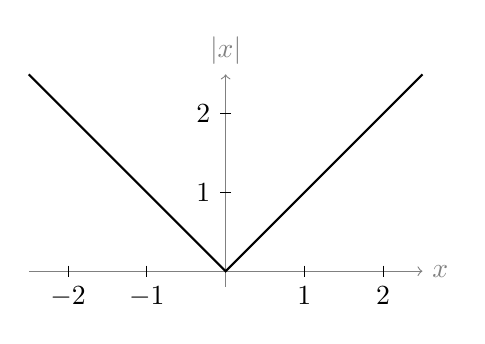
\begin{tikzpicture}[scale=1]
	\draw[->, gray] (-2.5,0) -- (2.5,0) node[right] {$x$};
	\draw[->, gray] (0,-.2) -- (0,2.5) node[above] {$|x|$};

	% BN-SRC-488: the two middle foreach items need explicit labels.
	\foreach \x/\xtext in {-2/-2, -1/-1, 1/1, 2/2}
	\draw[shift={(\x,0)}] (0pt,2pt) -- (0pt,-2pt) node[below] {{$\xtext$}};

	\foreach \y/\ytext in {1/1, 2/2}
	\draw[shift={(0,\y)}] (2pt,0pt) -- (-2pt,0pt) node[left] {{$\ytext$}};

	\draw[thick] (-2.5, 2.5)--(0,0)--(2.5, 2.5);
	\end{tikzpicture}
\end{center}
তাই সংজ্ঞাটির মোটামুটি অর্থ:
যুক্তির মান~$c$ থেকে
$\delta$-র কম দূরত্বে
বেছে নিলে (অর্থাৎ,
$|x - c| < \delta$)
তোমার “ভুল” $\epsilon$-এর
চেয়ে ছোট করা যায়
(অর্থাৎ,
$|g(x) - \ell| < \epsilon$)।

সীমার ধারণা সংজ্ঞায়িত হয়ে
গেলে অতিক্ষুদ্র রাশি একেবারেই
এড়ানো যায়। আমরা স্থির
করি, $c$-তে $f$-এর ঢাল:
\[
	{f}'(c) = \lim_{x \rightarrow 0}\left(\frac{f(c +x) - f(c)}{x}\right) \text{ যেখানে সীমাটি বিদ্যমান}.
\]
“যেখানে সীমাটি বিদ্যমান”
শর্তটি কেন চাই, তা বোঝা
গুরুত্বপূর্ণ। সরল উদাহরণ
হিসেবে এইমাত্র দেখা রেখাচিত্রের
$f(x) = |x|$ নাও।
স্পষ্টত, $f'(0)$-এর
সংজ্ঞা থাকে না: “ডান
দিক থেকে” $0$-এর
কাছে এলে ঢাল সব
সময় $1$; “বাঁ দিক
থেকে” এলে সব সময়
$-1$; তাই সীমাটি
বিদ্যমান নয়। সুতরাং
আমরা যোগ করতে পারি,
এমন সীমা থাকলে এবং
কেবল তখনই অপেক্ষক~$f$
বিন্দু~$x$-এ
\emph{অবকলনযোগ্য}।

\emph{সীমা}-র ধারণা
ব্যবহার করে অবকলন
কীভাবে সামলানো যায়,
তা আমরা দেখেছি।
একই ধারণা দিয়ে
\emph{অবিচ্ছিন্ন}
অপেক্ষকের ধারণাও
সংজ্ঞায়িত করা যায়।
(কার্যত ১৮১৭ সালেই
বোল্‌ৎসানো এটি
বুঝেছিলেন।)
অবিচ্ছিন্নতা নিয়ে
কোশি--ভাইয়ারস্ট্রাসের
ব্যাখ্যাটি এমন। মোটামুটি
বললে: কোনো বিন্দুতে
অপেক্ষক~$f$ অবিচ্ছিন্ন,
যদি ফলাফলে নির্দিষ্ট
নির্ভুলতা চাইলে
যুক্তির মানে যথেষ্ট
নির্ভুলতা দাবি করে
তা নিশ্চিত করা যায়।
আরও নির্ভুলভাবে:
$f$ বিন্দু~$c$-তে
অবিচ্ছিন্ন, যদি $x$
যখন $0$-এর দিকে
যায়, তখন
$f(c + x)$ ও
$f(c)$-এর পার্থক্যও
$0$-এর দিকে যায়।
অন্যভাবে, $f$ বিন্দু~$c$-তে
\emph{অবিচ্ছিন্ন}
যদি এবং কেবল যদি
$f(c) = \lim_{x \rightarrow c} f(x)$।

আর এগোলে সেটতত্ত্ব
ছেড়ে বাস্তব বিশ্লেষণে
ঢুকে পড়ব। তাই
এখানে থেমে মূল
কথাটি বলি।
ঊনবিংশ শতকে
গণিতবিদেরা
\emph{সীমা}-র
কঠোরভাবে সংজ্ঞায়িত
ধারণা ব্যবহার করে
অতিক্ষুদ্র রাশি
ছাড়াই কাজ করতে
শিখেছিলেন।

\end{document}
